\section{Timing Analysis}

\subsection{Introduction}
Timing analysis is the methodical analysis of a digital circuit to determine if the timing constraints imposed by components or interfaces are met. Typically, this means that you are trying to meet all set-up, hold, and pulse-width times requirement.\\ During designing there is a trade-offs between speed, area, power, and runtime according to the constraints set by the designer. However, a chip must meet the timing constraints to operate at the intended clock rate, so timing is the most important design constraint.

\subsection{Reasons for performing Timing Analysis}
\begin{itemize}
    \item To verify whether the design meets all the timing requirements.
    \item To verify that the design for all combinations of components over the entire specified operating environment at every time instance. 
    \item Timing analysis can also help with component selection.
\end{itemize}

\subsection{Types of Timing Analysis}

There are 2 type of Timing Analysis:
\begin{itemize}
    \item \textbf{Static Timing Analysis:} Checks static delay requirements of the circuit without any input or output vectors.
    \item \textbf{Dynamic Timing Analysis:} verifies functionality of the design by applying input vectors and checking for correct output vectors.
\end{itemize}

The basis of all timing analysis are the "Clock" and "Sequential component" (Flip-flop, Latches) of the design. Following are a few directives related to clock and Flip-Flop for Timing analysis.
\subsubsection{Clock directives}
\begin{itemize}
    \item Clock must be well understood parametrically and glitch-free.
    \item Timing analysis must ensure that any clock that is generated by the digital logic is clean, of bounded period \& duty cycle, and of a known phase relationship to other clock signals of interest.
    \item The clock must, for both high and low phases, meet the minimum pulse width requirements.
    \item Certain circuits, may require monitoring maximum jitter. Jitter might become a critical parameter, with higher clock speeds.
    \item When "passing" data from one clock edge to the other, one has to ensure that the worst-case duty cycle is used for the calculation. Remember: A frequent source of error is the designer assuming that every clock will have a 50\% duty cycle.
\end{itemize}
\clearpage
\subsubsection{Flip-Flop directives}
\begin{itemize}
    \item Make sure that all the parameters of Flip-Flops always met. The only exception is when synchronizers are used to synchronize asynchronous signals.
    \item For asynchronous presets and clears, Recovery and Removal constraints must be met.
    \item All setup and hold times are met for the earliest/latest arrival times for the clock.
    \item Setup times are generally calculated by designers and suitable margins can be demonstrated under test. Hold times, however, are frequently not calculated by designers.
    \item When passing data from one clock domain to another, ensure that there is either known phase relationships which will guarantee meeting setup and hold times or that the circuits are properly synchronized.    
\end{itemize}

\section{Static Timing Analysis (STA)}
\subsubsection{Definition}
Static timing analysis (STA) is a method of validating the timing performance of a design by checking all possible paths for timing violations under worst-case conditions. STA is more thorough because it checks the worst-case timing for all possible logic conditions, not just those sensitized by a particular set of test vectors. However, STA can only check the timing, not the functionality, of a circuit design unlike functional simulation.

\subsubsection{Description} 
In static timing analysis, the word static alludes to the fact that this timing analysis is carried out in an input-independent manner. There are huge numbers of logic paths inside a chip of complex design. The advantage of STA is that it performs timing analysis on all possible paths (whether they are real or potential false paths). However, it is worth noting that STA is not suitable for all design styles. It has proven efficient only for fully synchronous designs. Since the majority of chip design is synchronous, it has become a mainstay of chip design over the last few decades.\\
Static timing analysis involves following steps: 
\begin{enumerate}
    \item Breaks a design down into timing paths.
    \item Calculates the signal propagation delay along each path.
    \item Checks for violations of timing constraints inside the design and at the input/output interface.
\end{enumerate}

\subsection{Timing Paths}
When performing timing analysis, STA first breaks down the design into timing paths. Each timing path consists of the following elements:
\begin{enumerate}
    \item \textbf{Startpoint} The start of a timing path where data is launched by a clock edge or where the data must be available at a specific time. Every startpoint must be either an input port or a register clock pin.
    \item \textbf{Combinatorial logic network} Elements that have no memory or internal state. Combinatorial logic can contain AND, OR, XOR, and inverter elements, but cannot contain Flip-Flops, latches, registers, or RAM.
    \item \textbf{Endpoint} The end of a timing path where data is captured by a clock edge or where the data must be available at a specific time. Every endpoint must be either a register data input pin or an output port.
\end{enumerate}

\begin{figure}[H]
\begin{center}
\includegraphics[width=4.5in]{images/STAPaths.jpg}
\caption{Timing paths in a simple design example}
\label{STAPaths}
\end{center}
\end{figure}

A combinatorial logic cloud might contain multiple paths, as shown in the \figref{STAMultipath}. STA uses the longest path to calculate a maximum delay and the shortest path to calculate a minimum delay.

\begin{figure}[H]
\begin{center}
\includegraphics[width=4in]{images/STAMultipath.jpg}
\caption{Multiple timing paths in a combinatorial logic}
\label{STAMultipath}
\end{center}
\end{figure}

The STA tool analyzes all the paths from each and every startpoint to each and every endpoint and compares it against the constraint that (should) exist for that path. All paths should be constrained, most paths are constrained by the definition of the period of the clock, and the timing characteristics of the primary inputs and outputs of the circuit.
\clearpage
\subsection{Types of Timing Paths}
There are 4 types of Timing Paths:
\begin{enumerate}
    \item Data Path
    \item Clock Path
    \item Clock Gating Path
    \item Asynchronous Path 
\end{enumerate}

\begin{figure}[H]
\begin{center}
\includegraphics[width=4.5in]{images/STAPathTypes.jpg}
\caption{Types of timing paths in a combinatorial logic}
\label{STAPathTypes}
\end{center}
\end{figure}

Each of the Timing Paths, is explained with the help of \figref{STAPathTypes} in sections below.

\subsubsection{Data path}
Data path is a path from a clock input port or Clock pin, through the Flip-Flop/latch/memory (sequential cell), to the Data input pin of the sequential element.

\begin{itemize}
    \item Start Point: Input port of the design (for data from some external source) or,\\ Clock pin of the Flip-Flop/latch/memory (sequential cell).
    \item End Point: Data input pin of the Flip-Flop/latch/memory (sequential cell) or, \\ Output port of the design (for the data captured by some external sink).
\end{itemize}

\paragraph{Types of Data Paths}
With the combination of 2 types of Starting Points and 2 types of End Points, there are 4 types of Timing Paths, which are mentioned below:
\begin{enumerate}
    \item Input pin/port to Register(Flip-Flop). 
    \item Input pin/port to Output pin/port.
    \item Register (Flip-Flop) to Register (Flip-Flop)
    \item Register (Flip-Flop) to Output pin/port
\end{enumerate}

\begin{figure}[H]
\begin{center}
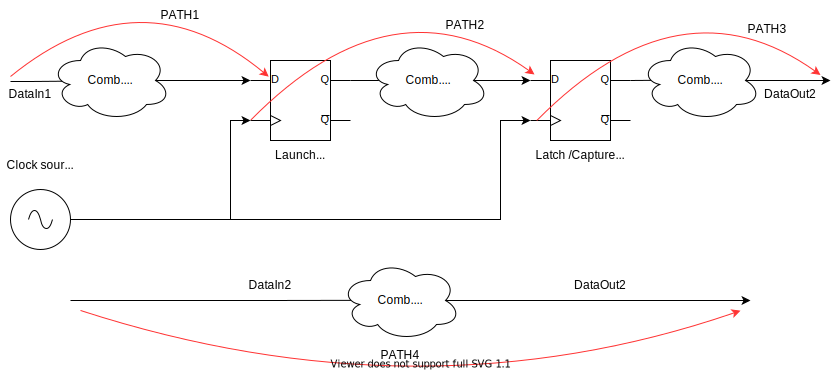
\includegraphics[width=\textwidth]{images/STADataPath.png}
\caption{Types of Data Paths in a combinatorial logic}
\label{STADataPath}
\end{center}
\end{figure}

\begin{itemize}
    \item PATH1- starts at an input port and ends at the data input of a sequential element. (Input port to Register)
    \item PATH2- starts at the clock pin of a sequential element and ends at the data input of a sequential element. (Register to Register)
    \item PATH3- starts at the clock pin of a sequential element and ends at an output port.(Register to Output port).
    \item PATH4- starts at an input port and ends at an output port. (Input port to Output port)
\end{itemize}

\subsubsection{Clock Path}
As per \figref{STAPathTypes}, Clock path is a path from a clock input port or cell pin, through one or more buffers or inverters, to the clock pin of a sequential element for data setup and hold checks. In between the Start point and the end point there may be lots of Buffers/Inverters/clock divider.

\begin{itemize}
    \item Start Point: Clock input port
    \item End Point: Clock pin of the Flip-Flop/latch/memory (sequential cell)
\end{itemize}

\subsubsection{Clock Gating Path}
As per \figref{STAPathTypes}, Clock path may be passed trough a gated element to achieve additional advantages. this type of clock path is called as gated clock path. Clock gating path is a path from an input port to a clock-gating element for clock gating setup and hold checks.

\begin{itemize}
    \item Start Point: Input port of the design
    \item End Point: Input port of clock-gating element.
\end{itemize}

\subsubsection{Asynchronous path}
As per \figref{STAPathTypes}, asynchronous path is a path from an input port to an asynchronous set or clear pin of a sequential element; for recovery and removal checks.

\begin{itemize}
    \item Start Point: Input port of the design
    \item End Point: Set/Reset/Clear pin of the Flip-Flop/latch/memory (sequential cell)
\end{itemize}

As you know that the functionality of set/reset pin is independent from the clock edge. Its level triggered pins and can start functioning at any instance of time. In other words, this path is not synchronous with the rest of the circuit and hence is called as Asynchronous path.

\subsection{Other types of Paths}
There are few more types of path which are used during timing analysis. Those are a subset of above mentioned paths with some specific characteristics. Other types of Paths include:
\begin{itemize}
    \item Critical path
    \item False Path
    \item Multi-cycle path
    \item Single Cycle path
    \item Launch Path
    \item Capture Path
    \item Longest Path ( Also know as Worst Path, Late Path, Max Path, Maximum Delay Path)
    \item Shortest Path ( Also Know as Best Path, Early Path, Min Path, Minimum Delay Path)
\end{itemize}

\iffalse
\subsubsection{Critical Path}
In short, I can say that the path which creates Longest delay is the critical path.
Critical paths are timing-sensitive functional paths. because of the timing of these paths is critical, no additional gates are allowed to be added to the path, to prevent increasing the delay of the critical path.
Timing critical path are those path that do not meet your timing. What normally happens is that after synthesis the tool will give you a number of path which have a negative slag. The first thing you would do is to make sure those path are not false or multicycle since it that case you can just ignore them.
Taking a typical example (in a very simpler way), the STA tool will add the delay contributed from all the logic connecting the Q output of one flop to the D input of the next (including the CLK-&gt;Q of the first flop), and then compare it against the defined clock period of the CLK pins (assuming both flops are on the same clock, and taking into account the setup time of the second flop and the clock skew). This should be strictly less than the clock period defined for that clock. If the delay is less than the clock period, then the "path meets timing". If it is greater, than the "path fails timing". The "critical path" is the path out of all the possible paths that either exceeds its constraint by the largest amount, or, if all paths pass, then the one that comes closest to failing.


False Path:
Physically exist in the design but those are logically/functionally incorrect path. Means no data is transferred from Start Point to End Point. There may be several reasons of such path present in the design.
Some time we have to explicitly define/create few false path with in the design. E.g for setting a relationship between 2 Asynchronous Clocks. 
The goal in static timing analysis is to do timing analysis on all true timing paths, these paths are excluded from timing analysis. 
Since false path are not exercised during normal circuit operation, they typically don't meet timing specification,considering false path during timing closure can result into timing violations and the procedure to fix would introduce unnecessary complexities in the design.
<li style="border-bottom: medium none; border-left: medium none; border-right: medium none; border-top: medium none;">There may be few paths in your design which are not critical for timing or masking other paths which are important for timing optimization, or never occur with in normal situation. In such case , to increase the run time and improving the timing result , sometime we have to declare such path as a False path , so that Timing analysis tool ignore these paths and so the proper analysis with respect to other paths. Or During optimization don't concentrate over such paths. One example of this. e.g A path between two multiplexed blocks that are never enabled at the same time. You can see the following picture for this.

<table align="center" cellpadding="0" cellspacing="0" class="tr-caption-container" style="margin-left: auto; margin-right: auto; text-align: center;"><tbody>
<tr><td style="text-align: center;"><a href="https://lh4.googleusercontent.com/-nb0f6wv3c60/TXCmhNOHMaI/AAAAAAAAACs/il_jOYJEH8U/s1600/false+path.bmp" imageanchor="1" style="margin-left: auto; margin-right: auto;"><img border="0" height="191" l6="true" src="https://lh4.googleusercontent.com/-nb0f6wv3c60/TXCmhNOHMaI/AAAAAAAAACs/il_jOYJEH8U/s400/false+path.bmp" width="400" /></a></td></tr>
<tr><td class="tr-caption" style="text-align: center;">False Path</td></tr>
</tbody></table><div style="border-bottom: medium none; border-left: medium none; border-right: medium none; border-top: medium none; text-align: left;">
Here you can see that False path 1 and False Path 2 can not occur at the same time but during optimization it can effect the timing of another path. So in such scenario, we have to define one of the path as false path.</div>
Same thing I can explain in another way (Note- Took snapshot from one of the forum). As we know that, not all paths that exist in a circuit are "real" timing paths. For example, let us assume that one of the primary inputs to the chip is a configuration input; on the board it must be tied either to VCC or to GND. Since this pin can never change, there are never any timing events on that signal. As a result, all STA paths that start at this particular startpoint are false. The STA tool (and the synthesis tool) cannot know that this pin is going to be tied off, so it needs to be told that these STA paths are false, which the designer can do by telling the tool using a "false_path" directive. When told that the paths are false, the STA tool will not analyze it (and hence will not compare it to a constraint, so this path can not fail), nor will a synthesis tool do any optimizations on that particular path to make it faster; synthesis tools try and improve paths until they "meet timing" - since the path is false, the synthesis tool has no work to do on this path.
Thus, a path should be declared false if the designer KNOWS that the path in question is not a real timing path, even though it looks like one to the STA tool. One must be very careful with declaring a path false. If you declare a path false, and there is ANY situation where it is actually a real path, then you have created the potential for a circuit to fail, and for the most part, you will not catch the error until the chip is on a board, and (not) working. Typically, false paths exists

from configuration inputs like the one described above
from "test" inputs; inputs that are only used in the testing of the chip,and are tied off in normal mode (however, there may still be some static timing constraints for the test mode of the chip)
from asynchronous inputs to the chip (and you must have some form of synchronizing circuit on this input) (this is not an exhaustive list, but covers the majority of legitimate false paths).
So we can say that false paths should NOT be derived from running the STA tool (or synthesis tool); they should be known by the designer as part of the definition of the circuit, and constrained accordingly at the time of initial synthesis.

MultiCycle Path:A multicycle path is a timing path that is designed to take more than one clock cycle for the data to propagate from the startpoint to the endpoint.

A multi-cycle path is a path that is allowed multiple clock cycles for propagation. Again, it is a path that starts at a timing startpoint and ends at a timing endpoint. However, for a multi-cycle path, the normal constraint on this path is overridden to allow for the propagation to take multiple clocks.
In the simplest example, the startpoint and endpoint are flops clocked by the same clock. The normal constraint is therefore applied by the definition of the clock; the sum of all delays from the CLK arrival at the first flop to the arrival at the D of the second clock should take no more than 1 clock period minus the setup time of the second flop and adjusted for clock skew.
By defining the path as a multicycle path you can tell the synthesis or STA tool that the path has N clock cycles to propagate; so the timing check becomes "the propagation must be less than N x clock_period, minus the setup time and clock skew". N can be any number greater than 1.

Few examples are
When you are doing clock crossing from two closely related clocks; ie. from a 30MHz clock to a 60MHz clock, 
Assuming the two clocks are from the same clock source (i.e. one is the divided clock of the other), and the two clocks are in phase. 
The normal constraint in this case is from the rising edge of the 30MHz clock to the nearest edge of the 60MHz clock, which is 16ns later. However, if you have a signal in the 60MHz domain that indicates the phase of the 30MHz clock, you can design a circuit that allows for the full 33ns for the clock crossing, then the path from flop30 -&gt; to flop60 is a MCP (again with N=2). 
The generation of the signal 30MHZ_is_low is not trivial, since it must come from a flop which is clocked by the 60MHz clock, but show the phase of the 30MHz clock.
Another place would be when you have different parts of the design that run at different, but related frequencies. Again, consider a circuit that has some stuff running at 60MHz and some running on a divided clock at 30MHz. 
Instead of actually defining 2 clocks, you can use only the faster clock, and have a clock enable that prevents the clocks in the slower domain from updating every other clock, 
Then all the paths from the "30MHz" flops to the "30MHz" flops can be MCP. 
This is often done since it is usually a good idea to keep the number of different clock domains to a minimum.

\fi

\subsection{Setup and Hold Time}
Say, an Input "DIN" and an external clock "CLK" are buffered and passed through a combinational logic to reach a synchronous input and a clock input of a D Flip-Flop (say positive edge triggered). To capture the data correctly at D Flip-Flop, data should be present at the time of positive edge of clock signal at the Clk pin.

\begin{figure}[H]
\begin{center}
\includegraphics[width=4.5in]{images/STASetupHold.jpg}
\caption{Setup and Hold Time of the system}
\label{STASetupHold}
\end{center}
\end{figure}

Where,
\begin{itemize}
    \item \(T_{pdDIN}\): Propagation delay of DIN
    \item \(T_{pdClk}\): Propagation delay of CLK
    \item \(T_{s(in)}\): Setup time of the system
    \item \(T_{h(in)}\): Hold time of the system
    \item \(T_{s}\): Setup time of the D Flip-Flop
    \item \(T_{h)}\): Hold time of the D Flip-Flop
    \item DIN: System input
    \item CLK: System clock
\end{itemize}

In an ideal case, the setup and hold time would be zero. But still, 2 cases would arise.
\begin{itemize}
    \item \(T_{pdDIN} > T_{pdClk}\): For a successful capture, the data should be stable for \(T_{pdDIN} - T_{pdClk} = T_{S(in)}\) time at DIN pin before the positive clock edge at CLK pin. This Time "\(T_{s(in)}\)" is know as Setup time of the System.
    \item  \(T_{pdDIN} < T_{pdClk}\): For a successful capture, the data should remain stable for "\(T_{h(in)}\)" time at DIN pin after the positive clock edge at CLK pin. This time "\(T_{h(in)}\)" is know as Hold Time of the System.
\end{itemize}

From the above conditions, both the conditions are mutually exclusive. But we have to consider few more things in this.

\begin{itemize}
    \item Worst case and best case (Max delay and min delay): Considering the environmental \& Operating(PVT) conditions, analysis is performed for the worst case (max delay) and best case (min delay).
    \item Shortest Path or Longest path (Min Delay and Max delay): If a combinational logic has multiple paths, then the analysis is performed for the shortest path (min delay) \& longest path (max delay).
\end{itemize}

In other words,
\begin{itemize}
    \item \(T_{pdDIN(max)} > T_{pdClk(min)}\): \[Setup Time = T_{pdDIN(max)} - T_{pdClk(min)} \]
    \item  \(T_{pdDIN(min)} < T_{pdClk(max)}\): \[Hold Time = T_{pdClk(max)} - T_{pdDIN(min)} \]
\end{itemize}

When a hold check is performed we have to consider two things:
\begin{itemize}
    \item Minimum delay along the data path
    \item Maximum delay along the clock path 
\end{itemize}

When a setup check is performed we have to consider two things:
\begin{itemize}
    \item Maximum delay along the data path
    \item Minimum delay along the clock path 
\end{itemize}

\subsubsection{Definition}

\textbf{Setup time} is the minimum amount of time the data signal should be held steady before the clock event so that the data are reliably sampled by the clock. In other words, Setup time is the minimum amount of time required for the input of a Flip-Flop to be stable before the clock edge comes along.\\ 

\textbf{Hold time} is the minimum amount of time the data signal should be held steady after the clock event so that the data are reliably sampled. In other words, Hold time is the minimum amount of time required for the input of a Flip-Flop to be stable after the clock edge comes along.\\  

\begin{figure}[H]
\begin{center}
\includegraphics[width=4.5in]{images/STASetupHold2.jpg}
\caption{Setup and Hold Time Definitions}
\label{STASetupHold2}
\end{center}
\end{figure}

As the D Flip-Flop can be constructed with various implementations like, JK Flip-Flop, master slave Flip-Flop, Using 2 D type latches etc. Since, the internal circuitry is different for each type of Flip-Flop, the Setup and Hold time is different for every Flip-Flop.

\subsection{Setup and Hold Violation}
If the data is not stable before the Setup time calculated from active edge of the clock, there is a Setup violation at that Flip-Flop.\\ 
If the data is not stable after Hold time calculated from active edge of the clock, there is a hold violation at that Flip-Flop.

\begin{figure}[H]
\begin{center}
\includegraphics[width=4.5in]{images/STASetupHoldViolation.jpg}
\caption{Setup and Hold Time Violation}
\label{STASetupHoldViolation}
\end{center}
\end{figure}

\figref{TimingFF} is used to explain the Setup and Hold time Violation. The register transfer level is implemented on the hardware with VLSI technologies. The actual implemented hardware looks exactly like this instance of RTL from \figref{TimingFF}. This representation is the most commonly occurring structure inside any digital design hardware implementations. Two registers working on a single clock launching and capturing data with some form of combinatorial logic sitting between the two.

\begin{figure}[H]
\begin{center}
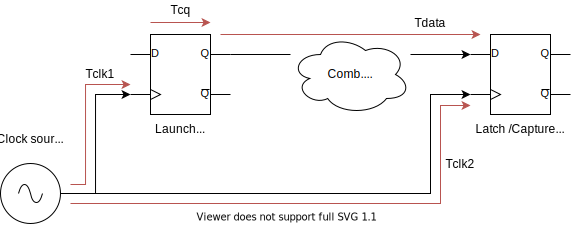
\includegraphics[width=\textwidth]{images/TimingFF.png}
\caption{Basic concepts of Timing Analysis}
\label{TimingFF}
\end{center}
\end{figure}

\begin{figure}[H]
\begin{center}
\includegraphics[width=\textwidth]{images/TimingDiaFF.png}
\caption{Timing Diagram}
\label{TimingDiaFF}
\end{center}
\end{figure}
    

\iffalse
Timing Diagram made from Wavedrom: https://wavedrom.com/
Source Code for timing diagram generation:
{signal: [
  {name: 'Source clk', wave: 'lh...l...h...l..'},
  {name: "TCLK1",   wave: "050......50....."},
  {name: 'FF1.clk', wave: 'l.h...l...h...l.'},
  {name: "Tcq",   wave: "l.50......50...."},
  {name: 'FF1.Q', wave: 'x..2...x...2...x', data: 'ValidData ValidData'},
  {name: "Tdata1",   wave: "l..50......5.0.."},
  {name: "Arrival time",   wave: "l5..0....5...0..", data: 'ArrivalTime1 ArrivalTime2'},
  {name: 'Source clk', wave: 'lh...l...h...l..'},  
  {name: "TCLK2",   wave: "07.0.....7.0...."},
  {name: 'FF2.clk', wave: 'l..h...l...h...l'},  
  {name: "Setup Hold",   wave: "0.340.....340...", data: 'Ts Th Ts Th'},  
  {name: "Setup Slack",   wave: "0...9.....0.....", data: 'SetupSlack'},  
  {name: "Hold Slack",   wave: "0...........90.."}, 
  {name: 'FF2.D', wave: 'x...2...x....2..',  data: 'ValidData ValidData'}
]}

Source code for recovery and removal timing
{signal: [
  {name: 'Clock', wave: 'l....h.....'},
  {name: "Asynchronous Reset",   wave: "h.l.....h.."},
  {name: "Recovery & Removal",   wave: "l..9.9.0...", data: 'Trec Trem'}
]}

\fi
\clearpage
Following are the basic concepts of Timing Analysis \& Setup, Hold Violation:
\begin{itemize}
    \item \textbf{Launch Edge} the edge which "launches" the data from source register.
    \item \textbf{Latch/Capture Edge} the edge which "Latches/Captures" the data at destination register (with respect to the launch edge).
    \item \textbf{Launch Flip-Flop} the Flip-Flop which "launches" the data on the launch edge.
    \item \textbf{Latch/Capture Flip-Flop} the Flip-Flop which "Latches/Captures" the data on the Latch/Capture edge.
    \item \textbf{Data Arrival Time} The time for data to arrive at destination register’s D input. Setup time is not considered while calculating Data Arrival Time.
    \[Data Arrival Time = launch edge + Tclk1 + Tcq +Tdata\]
    \item \textbf{Data Required Time (Setup)} The minimum time required for the data to get latched into the destination register. 
    \[Data Required Time Setup = Clock Arrival Time - Tsu - Setup Uncertainty\]
    \item \textbf{Data Required Time (Hold)} The minimum time required for the data to get latched into the destination register
    \[Data Required Time Hold = Clock Arrival Time + Th + Hold Uncertainty \]
    \item \textbf{Setup Slack} The margin by which the setup timing requirement is met. It ensures launched data arrives in time to meet the latching requirement. One reason for negative slack might be a large combinatorial logic. One of the Solutions: One more Flip-Flop can be added by breaking combinatorial logic into 2 parts. Setup slack is calculated on the next clock edge. And hence, it is dependant on clock frequency. If the value of the setup slack is 
    \begin{itemize}
        \item positive:  there is no setup violation.
        \item negative: (Data Arrival Time > Data Required Time(Setup)) Timing requirement is not met.
    \end{itemize}

    \[Setup Slack = Data Required Time(Setup) - Data Arrival Time\]
    Where,
    \begin{itemize}
        \item Arrival time (max) = clock delay FF1 (max) + Clk2Q delay FF1 (max) + comb. Delay( max)
        \item Required time = clock adjust + clock delay FF2(min) - Set up time FF2
        \item Clock adjust = clock period (since setup is analyzed at next edge)
    \end{itemize}

    \item \textbf{Hold Slack} The margin by which the hold timing requirement is met. It ensures latch data is not corrupted by data from another launch edge. It also prevents "double-clocking". Hold slack is calculated on a single clock edge. And hence, it is not dependant on clock frequency. If the value of the Hold slack is 
    \begin{itemize}
        \item positive: There is no setup violation. Data is not corrupted by the data from another launch edge.
        \item negative: Timing requirement is not met. Data is corrupted by the data from another launch edge.
    \end{itemize}
    \[ Hold slack = Data Arrival Time - Data Required Time(Hold)\]
    Where,
    \begin{itemize}
        \item Arrival time (min) = clock delay FF1 (min) + Clk2Q delay FF1 (min) + comb. Delay( min)
        \item Required time = clock adjust + clock delay FF2 (max) + hold time FF2
        \item Clock adjust = 0 (since hold is analyzed at same edge)
    \end{itemize}
    \item \textbf{Maximum Clock Frequency}: is the reciprocal of maximum delay out of (register to register, clk to q, \& pin to pin delays\\ 
    MaxClkFreq = 1 / max(Reg2Reg delay, Clk2Q delay, Pin2Pin delay). Where,
    \begin{itemize}
        \item Reg2Reg Delay = Clk2Q delay of FF1(max) + comb delay(max) + setup time of FF2.
        \item Clk2Q Delay = Clock delay w.r.t FF(max) + Clk2Q delay of FF1 (max) + comb delay (max)
        \item Pin2Pin delay = Comb delay between input pin to output pin (max)
    \end{itemize}             
    \item \textbf{Removal} The minimum time an asynchronous signal must be de-asserted AFTER clock edge.
    \item \textbf{Recovery} The minimum time an asynchronous signal must be de-asserted BEFORE clock edge.
\end{itemize}

\begin{figure}[H]
\begin{center}
\includegraphics[width=\textwidth]{images/TimingRR.png}
\caption{Timing Diagram for Removal and Recovery Time}
\label{TimingRR}
\end{center}
\end{figure}

\clearpage

Formulae
\begin{itemize}
    \item \textbf{Setup Calculations} 
    \begin{itemize}
        \item Setup Slack = Data Required Time(Setup) - Data Arrival Time
        \item Arrival time (max) = clock delay FF1 (max) + Clk2Q delay FF1 (max) + comb. Delay( max)
        \item Required time = clock adjust + clock delay FF2(min) - Set up time FF2
        \item Clock adjust = clock period (since setup is analyzed at next edge)
    \end{itemize}

    \item \textbf{Hold Calculation}
    \begin{itemize}
        \item Hold slack = Data Arrival Time - Data Required Time(Hold)
        \item Arrival time (min) = clock delay FF1 (min) + Clk2Q delay FF1 (min) + comb. Delay( min)
        \item Required time = clock adjust + clock delay FF2 (max) + hold time FF2
        \item Clock adjust = 0 (since hold is analyzed at same edge)
    \end{itemize}

    \item \textbf{Maximum Clock Frequency}:
    \begin{itemize}
        \item MaxClkFreq = 1 / max(Reg2Reg delay, Clk2Q delay, Pin2Pin delay)
        \item Reg2Reg Delay = Clk2Q delay of FF1(max) + comb delay(max) + setup time of FF2.
        \item Clk2Q Delay = Clock delay w.r.t FF(max) + Clk2Q delay of FF1 (max) + comb delay (max)
        \item Pin2Pin delay = Comb delay between input pin to output pin (max)
    \end{itemize}
\end{itemize}

\clearpage

\subsection{Delay Calculation}
After breaking down a design into a set of timing paths, an STA tool calculates the delay along each path. The total delay of a path is the sum of all cell and net delays in the path. \textbf{Cell delay} is the amount of delay from input to output of a logic gate in a path. In the absence of back-annotated delay information from an SDF file, the tool calculates the cell delay from delay tables provided in the logic library for the cell.

Typically, a delay table lists the amount of delay as a function of one or more variables, such as input transition time and output load capacitance. From these table entries, the tool calculates each cell delay.

Net delay is the amount of delay from the output of a cell to the input of the next cell in a timing path. This delay is caused by the parasitic capacitance of the interconnection between the two cells, combined with net resistance and the limited drive strength of the cell driving the net.

STA then checks for violations of timing constraints, such as setup and hold constraints:

A setup constraint specifies how much time is necessary for data to be available at the input of a sequential device before the clock edge that captures the data in the device. This constraint enforces a maximum delay on the data path relative to the clock edge.
A hold constraint specifies how much time is necessary for data to be stable at the input of a sequential device after the clock edge that captures the data in the device. This constraint enforces a minimum delay on the data path relative to the clock edge.
The following example shows how STA checks setup and hold constraints for a Flip-Flop

\clearpage

\textbf{Reset signal}
A Reset signal is required to initialize a hardware design for system operation and to force a hardware into a known state for simulation. There are two types of reset.

Synchronous Reset: A synchronous reset signal will only reset the state of the Flip-Flop on the active edge of the clock.
 
Asynchronous Reset: An asynchronous reset will reset the state of the Flip-Flop asynchronously i.e. no matter what the clock signal is. This is considered as high priority signal and system reset happens as soon as the reset assertion is detected.


Synchronous reset is good as everything's predictable. But with asynchronous resets should not cause issues only if the recovery and removal conditions are met. Right?

Asynchronous resets have a number of drawbacks:
\begin{enumerate}
    \item They may cause metastability in Flip-Flops, leading to a non-deterministic behavior.
    \item The asynchronous resets may incur reliability problems. 
\end{enumerate}

Steps to Using TimeQuest
\begin{enumerate}
    \item Generate timing netlist
    \item Read SDC file
    \item Update timing netlist
    \item Generate timing reports
\end{enumerate}

\subsection{Timing Constraints}
\subsubsection{About XDC Constraints}
XDC constraints are a combination of:
\begin{itemize}
    \item Industry standard Synopsys Design Constraints (SDC), and
    \item Xilinx proprietary physical constraints
\end{itemize}

XDC constraints have the following properties:
\begin{itemize}
    \item They are not simple strings, but are commands that follow the Tcl semantic.
    \item They can be interpreted like any other Tcl command by the Vivado Tcl interpreter.
    \item They are read in and parsed sequentially the same as other Tcl commands.
\end{itemize}

\subsubsection{Recommended Constraints Sequence}
\begin{itemize}
    \item Timing Assertions Section
    \begin{itemize}
        \item Primary clocks
        \item Virtual clocks
        \item Generated clocks
        \item Clock Groups
        \item Input and output delay constraints
    \end{itemize}
    \item Timing Exceptions Section
    \begin{itemize}
        \item False Paths
        \item Max Delay / Min Delay
        \item Multicycle Paths
        \item Case Analysis
        \item Disable Timing
    \end{itemize}
    \item Physical Constraints Section
    \begin{itemize}
        \item located anywhere in the file, preferably before or after the timing constraints
        \item or stored in a separate XDC file 
    \end{itemize}
\end{itemize}

\subsubsection{create\_clock} 
A primary clock is a board clock that enters the design either through an input port, or A gigabit transceiver output pin (for example, a recovered clock). A primary clock can be defined only by the create\_clock command. A primary clock must be attached to a netlist object. This netlist object represents the point in the design from which all the clock edges originate and propagate downstream on the clock tree. create\_clock constraint constrains all the reg to reg paths running on a particular clock.\\
\centerline{ex. create\_clock -period 10 [get\_ports clk] -waveform(o) "duty cycle"}
\paragraph{virtual clock} A virtual clock is a clock without any source. In other words, a clock that has been defined, but has not been associated with any pin/port.
TO constrain virtual clocks, no arguments like "get\_ports" are used.\\
\centerline{ex. create\_clock -period 10 -waveform(o) "duty cycle"}

\subsubsection{set\_clock\_uncertainty}
Modelling clock skew Uncertainty models the maz delay difference between clock network branches (Clock skew)\\    
\centerline{clock Uncertainty = clock skew + jitter + time\_margin}
\centerline{set\_clock\_uncertainty -setup 0.5 [get\_ports clk]}

\subsubsection{set\_clock\_latency}
Modelling the latency or latency or insertion delay. Latency is modelled in 2 parts: 
\begin{itemize}
    \item Source Latency : delay between clock source to clock port External to the 
    \item Network Latency : delay between clock port to register clock pin
    \item Total Latency = Source Latency + Network Latency
\end{itemize}
\centerline{Ex. set\_clock\_latency -source(Source Latency) 0.2 -max(Network Latency) 0.3 [get\_ports clk]}

\subsubsection{set\_clock\_transition}
Modelling transition time. Models the rise \& fall time on clock waveform.\\
\centerline{ex. set\_clock\_transition -max 0.6 [get\_clocks clk]}

\subsubsection{set\_input\_delay}
Constraining input paths. data arrival time.\\  
\centerline{ex. set\_input\_delay -max 0.6 -clock vclk [get\_ports A]}

\subsubsection{set\_output\_delay}
maximum output delay: amount of delay for the external designs capturing clock edge.\\
\centerline{ex. set\_output\_delay -max 0.45 -clock vclk1 [get\_ports B]}

\subsubsection{set\_false\_path}
Tells STA tool that a particular path is not used and should not be considered for the analysis.\\
\centerline{ex. set\_false\_path -from [get\_clocks clk1] -to [get\_clocks clk2]} 

\subsubsection{set\_clock\_groups}
Tells STA tool that a particular path is not used and should not be considered for the analysis.\\
\centerline{ex. set\_clock\_groups -logically\_exclusive -group clk1 -group clk2}





\subsubsection{Timing effects}
Timing effects of 
\begin{itemize}
    \item Transition time at input ports\\
    \centerline{set\_input\_transition -max 0.12 [get\_ports A]}
    \item Capacitive loading on output ports\\
    \centerline{set\_load -max  [expr {30.0/1000}] [get\_ports B]}
\end{itemize}
